\section{Download rates}
	As mentioned in section \ref{sec:approach}, longer circuits often result in lower download speeds. To confirm this, besides measuring the CPU speed we simultaneously measured the download rate. For each of the six test settings, we generated a graph just as we did with the CPU measurements. Since three hops with crypto did not work, these two runs are with encryption disabled .
	
	\subsection{Download rate when downloading directly}
		When downloading directly, the CPU can be almost fully dedicated to consume the data input stream.
		Since there is no decryption needed, we expected a high download rate. This was also confirmed when running the test, as can be seen in figure \ref{fig:download_rate_anonmode_off}. With peaks of over 1000 KB/s the download was completed in one minute.
		
			\begin{figure*}[!htb]
				\centering
				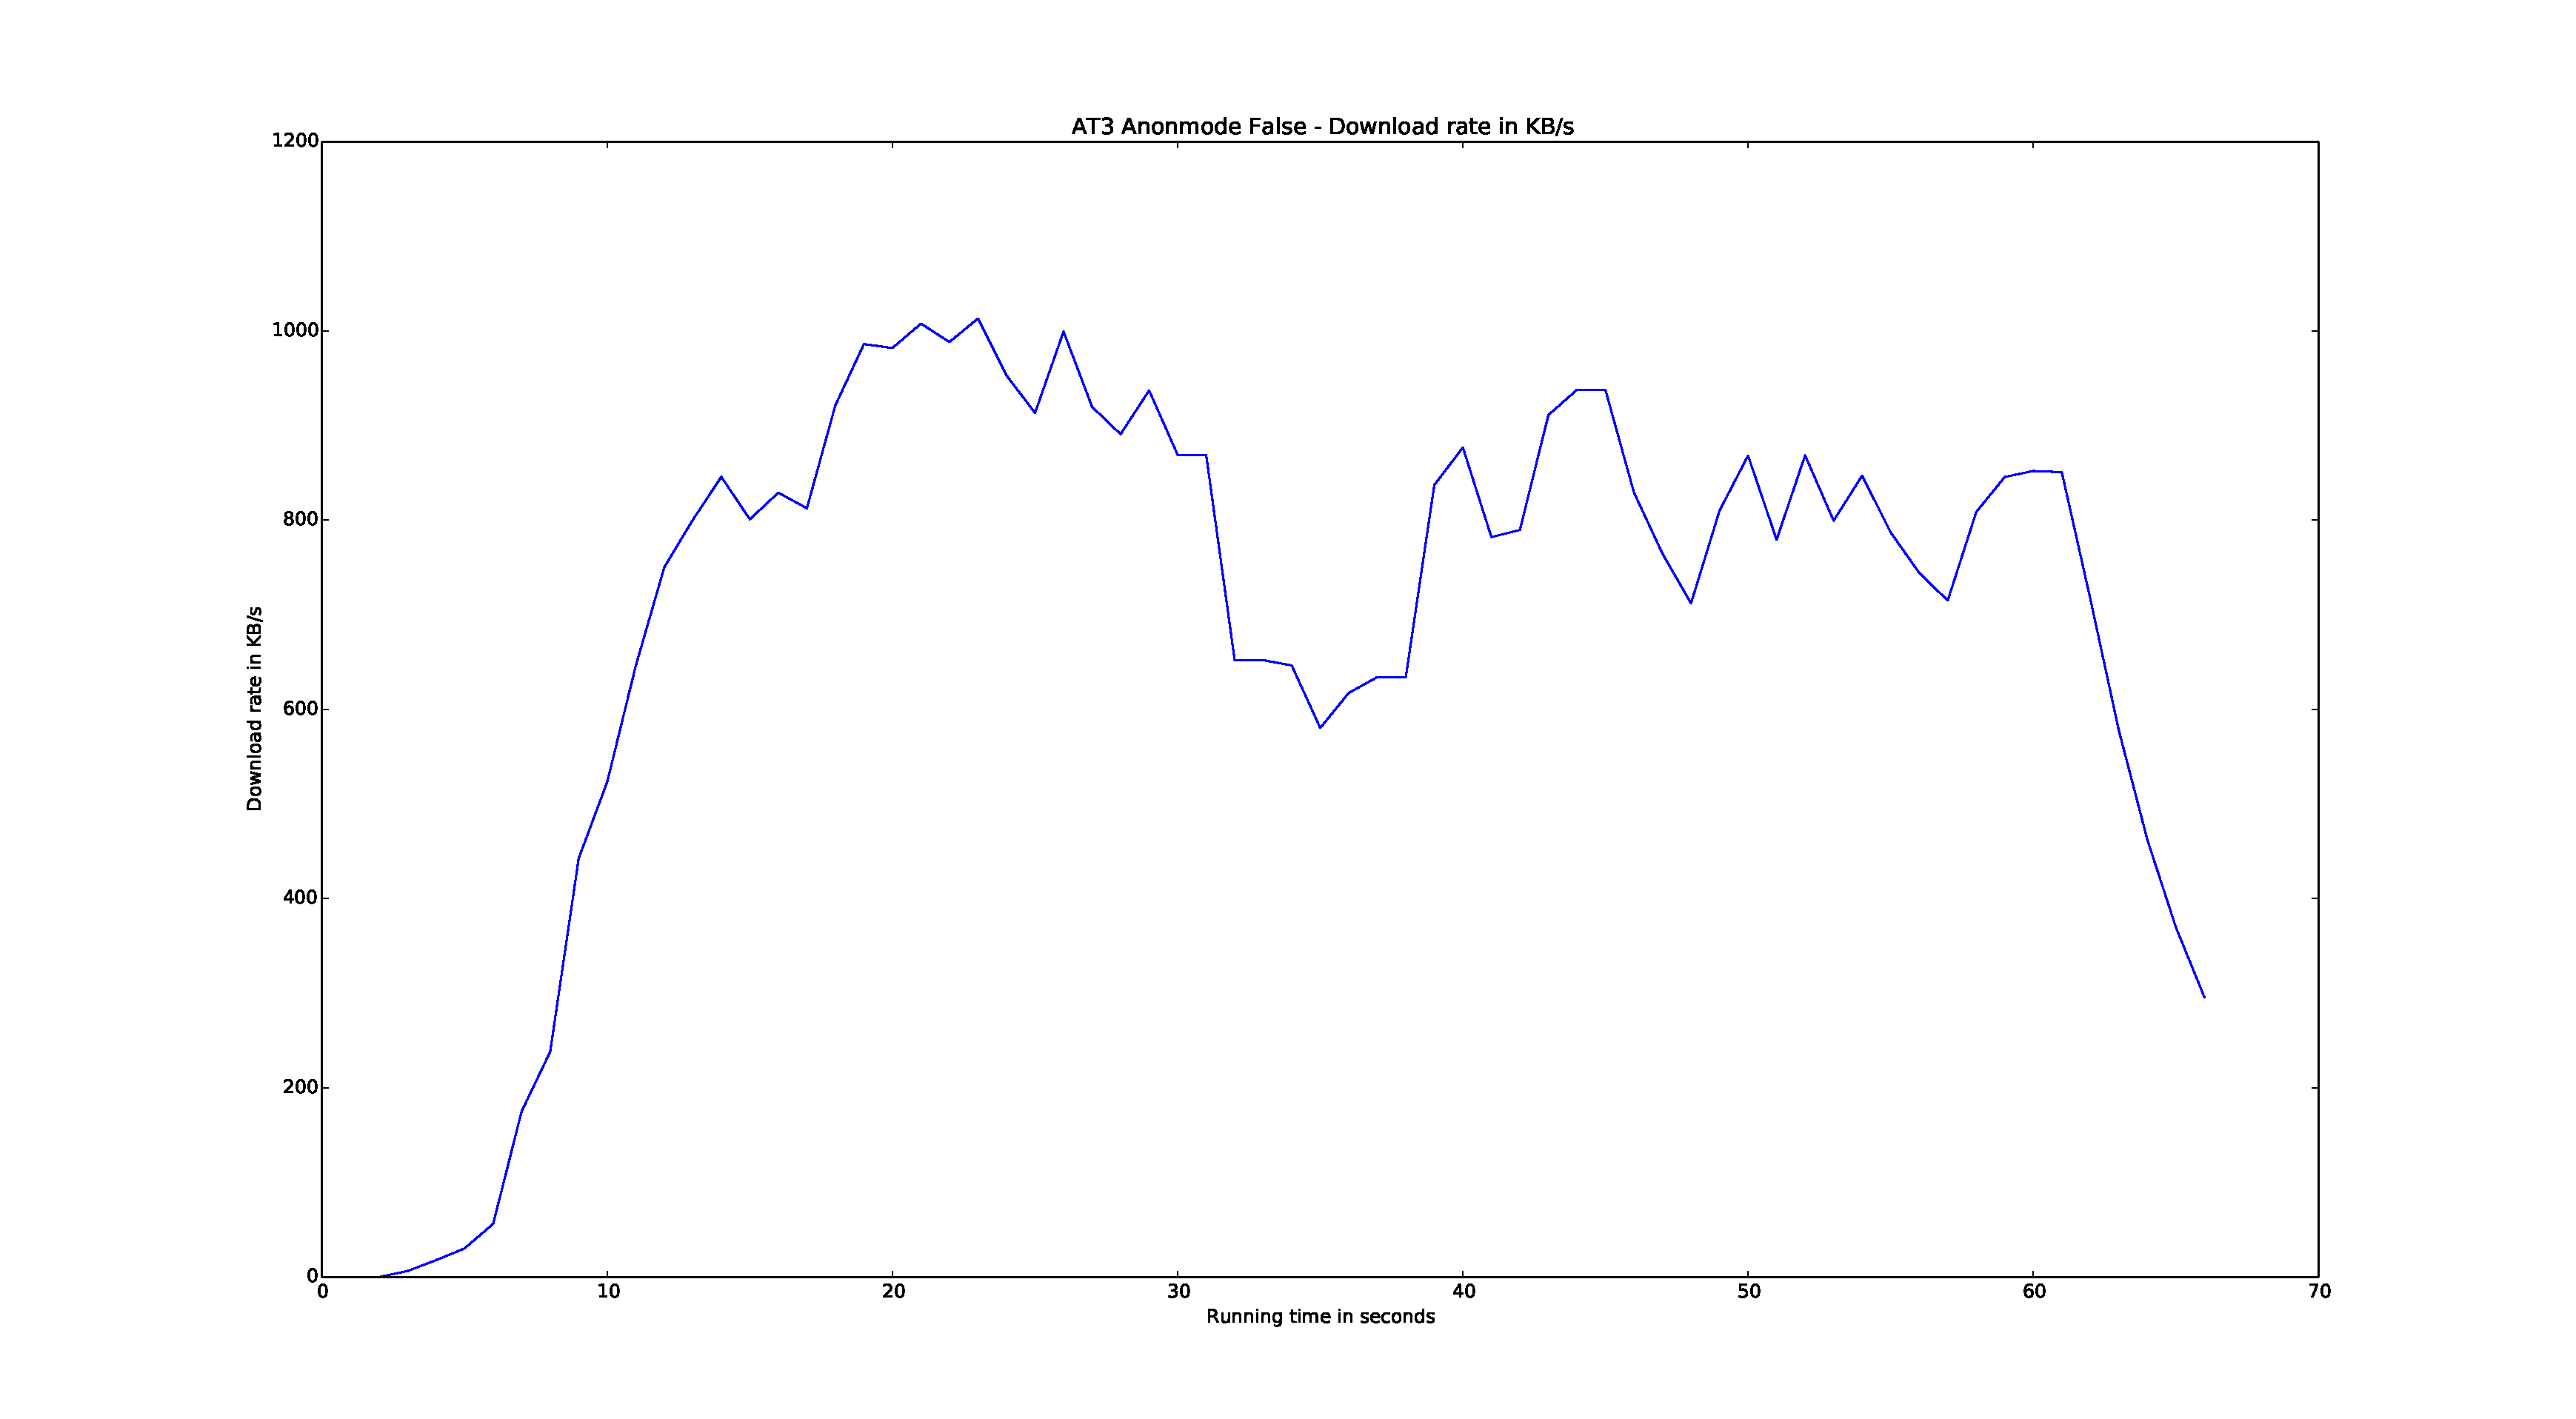
\includegraphics[width=\textwidth]{graphics/download_rate_anonmode_off.pdf}
				\caption{The download rate of downloading a 50 MB over one hop with one circuit.}
				\label{fig:download_rate_anonmode_off}
			\end{figure*}
			
		\subsection{Download rate when downloading over 1 hop with 1 circuit}
			As this test run downloads just over one hop, we expect to hit high download rates. The download rates themselves are expected to fluctuate a lot, because it is just one circuit providing the data. These fluctuations were indeed observed during the test run, visible in figure \ref{fig:download_rate_1_hop_1_circuit}.
			
			\begin{figure*}[!htb]
				\centering
				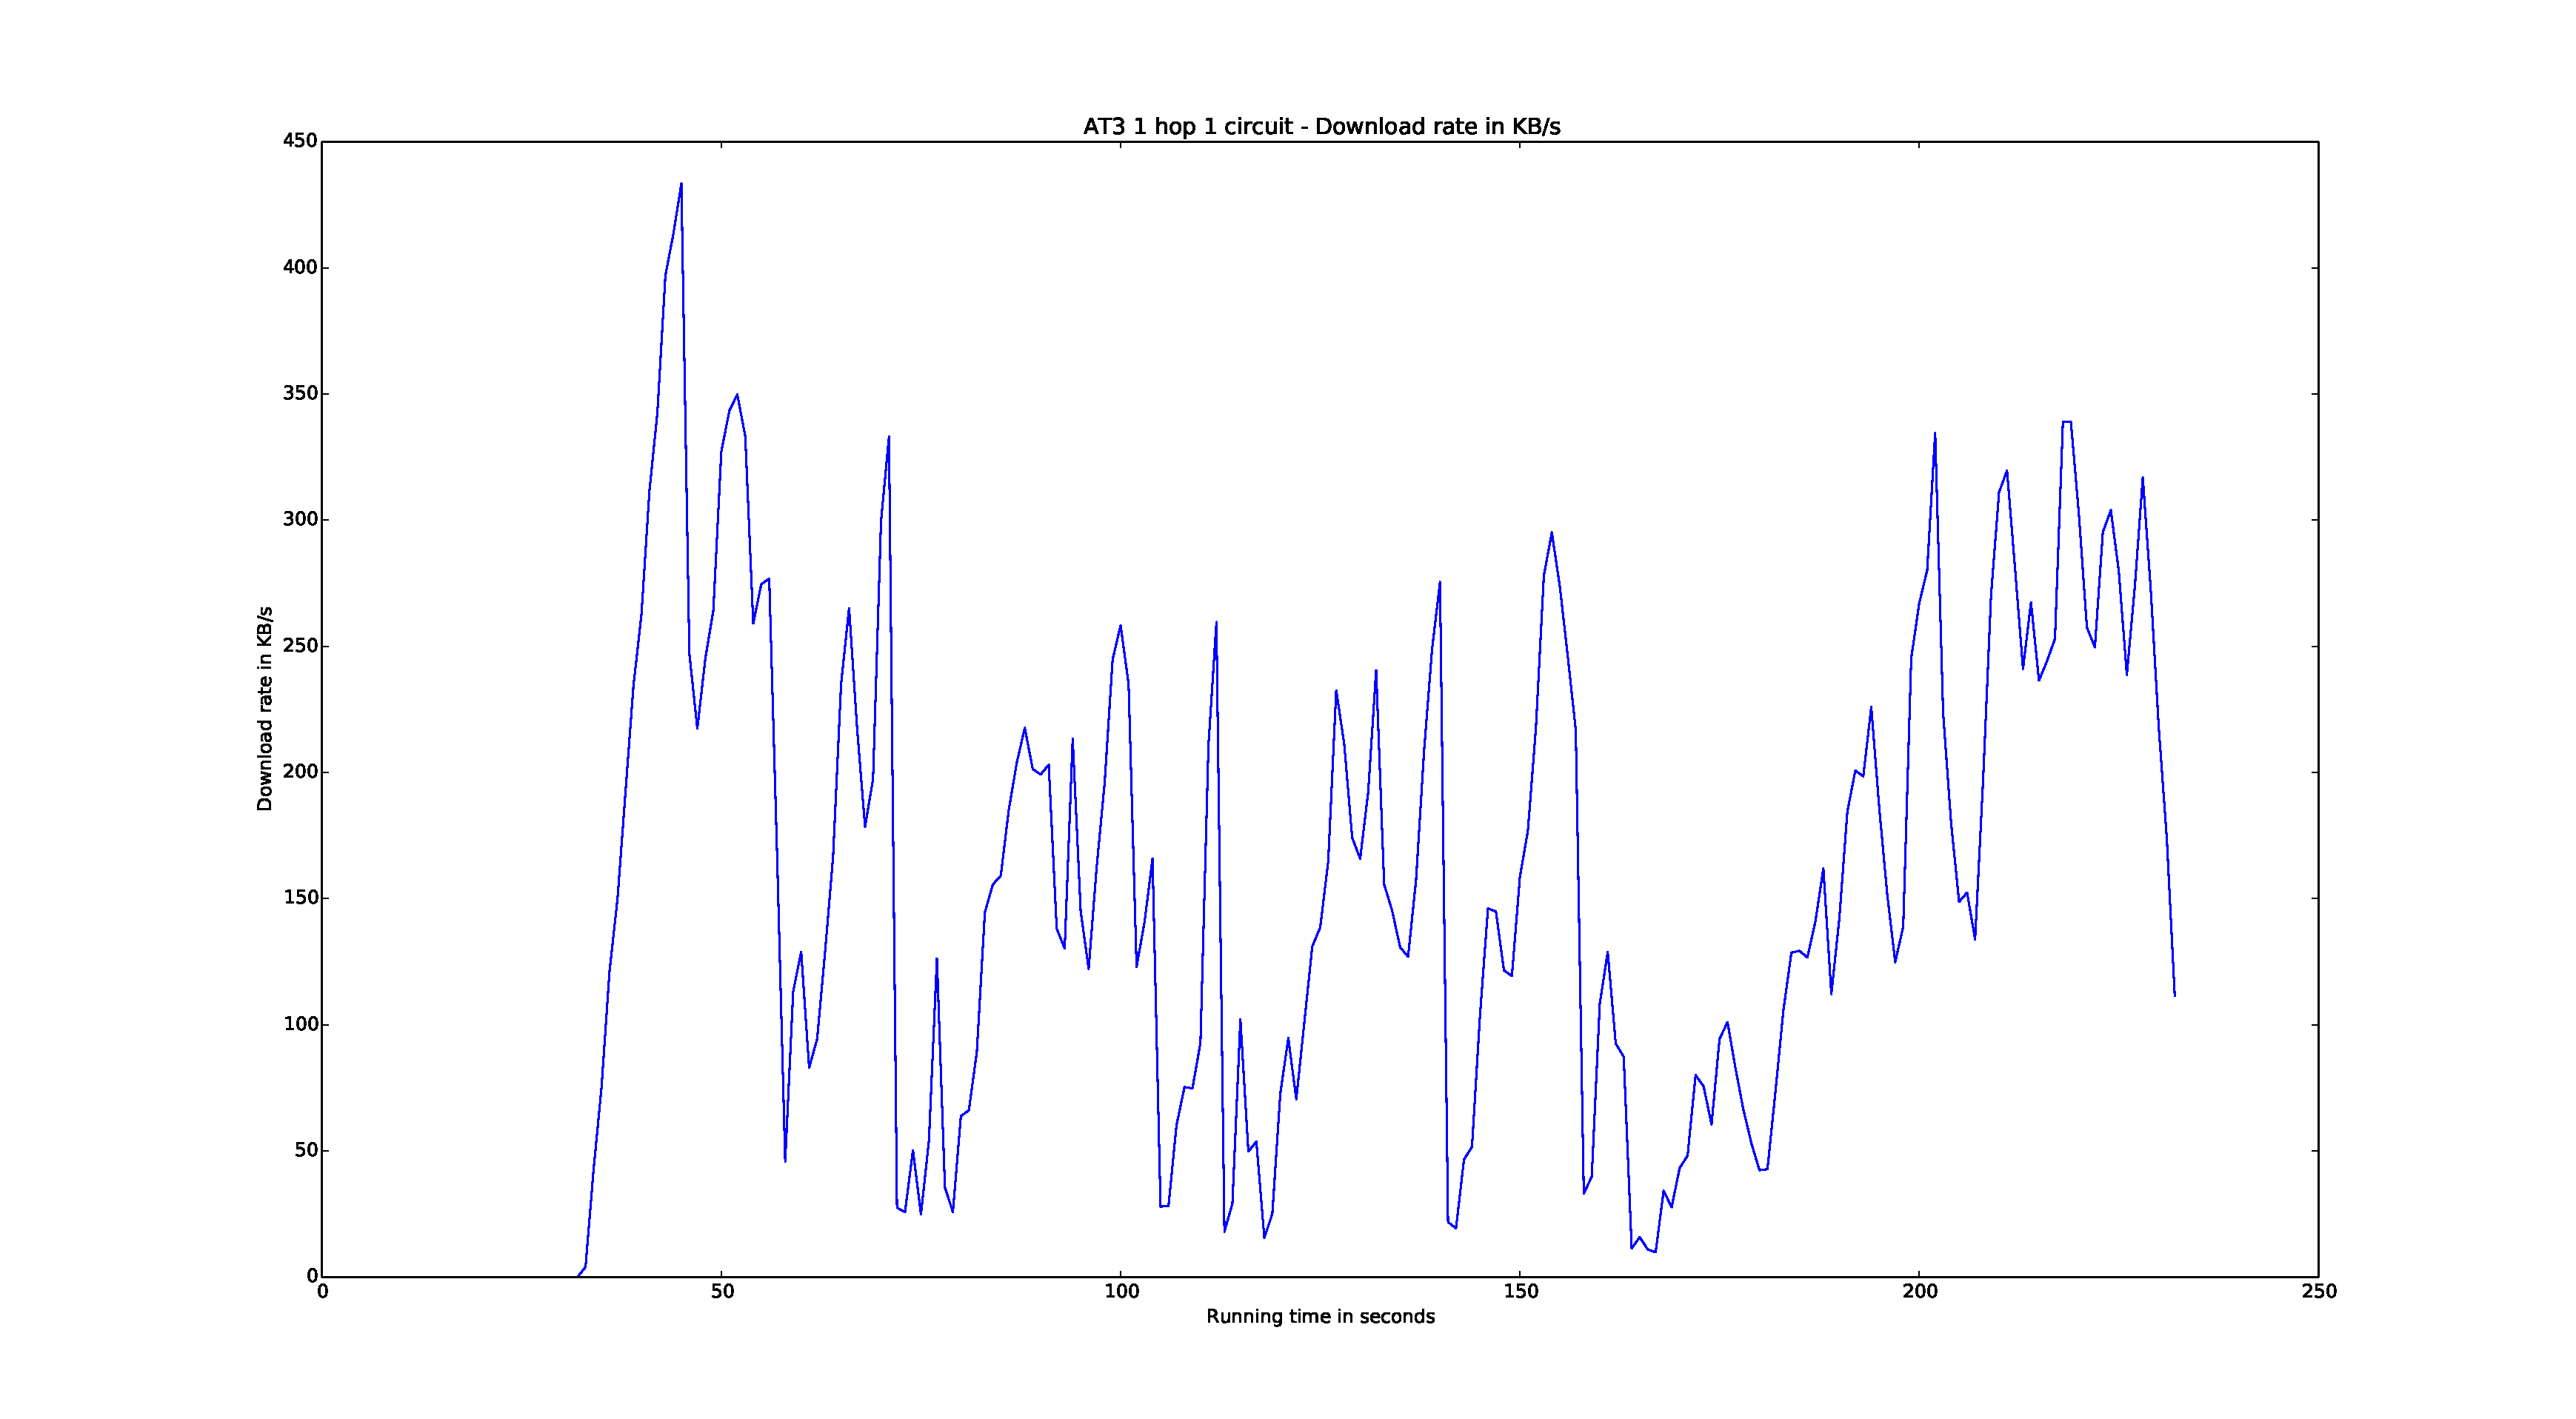
\includegraphics[width=\textwidth]{graphics/download_rate_1_hop_1_circuit.pdf}
				\caption{The download rate of downloading a 50 MB over one hop with one circuit.}
				\label{fig:download_rate_1_hop_1_circuit}
			\end{figure*}
			
		\subsection{Download rate when downloading over 1 hop with 3 circuits}
			When download over three circuits we expect the download rate to be more stable. The download rate should be about the same as with one hop, and should be overall even slightly higher. Figure \ref{fig:download_rate_1_hop_3_circuits} shows the download rates during the test run. Here we can see that the download indeed took less time, meaning the overall rate was faster.
			
			\begin{figure*}[!htb]
				\centering
				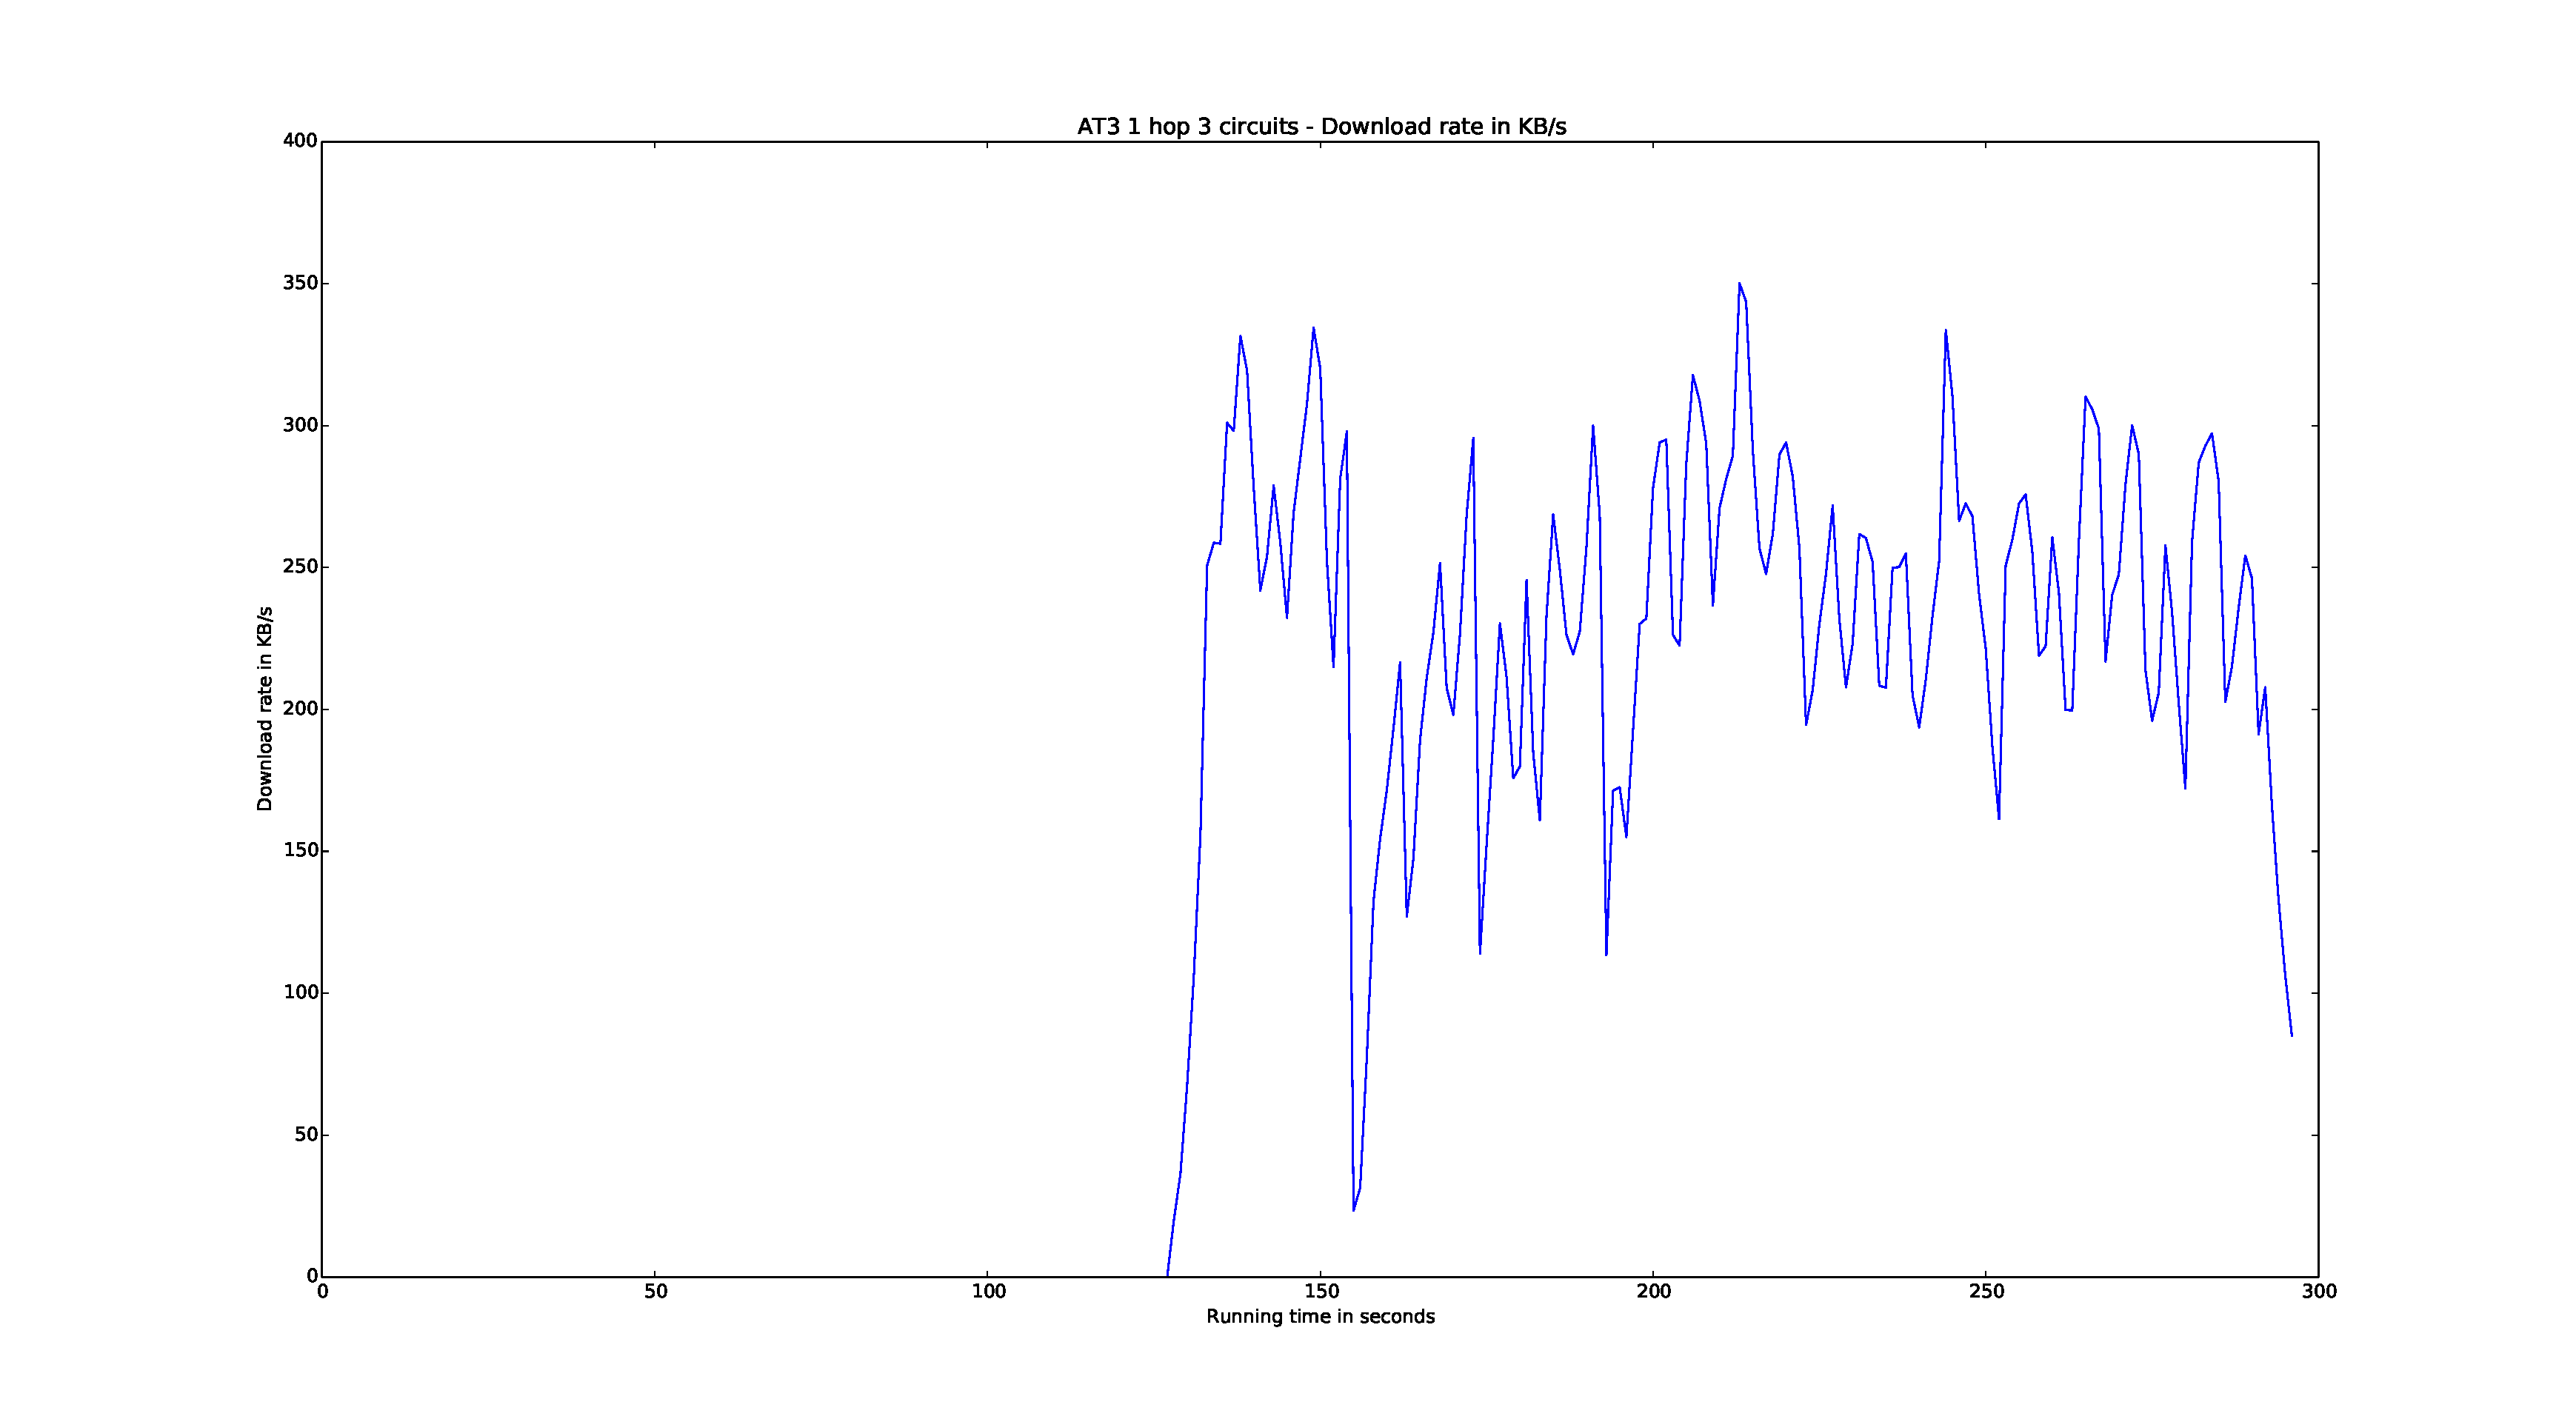
\includegraphics[width=\textwidth]{graphics/download_rate_1_hop_3_circuits.pdf}
				\caption{The download rate of downloading a 50 MB over one hop with three circuits.}
				\label{fig:download_rate_1_hop_3_circuits}
			\end{figure*}
			
		\subsection{Download rate when downloading over 3 hops with 1 circuit}
			As described in subsection \ref{ssec:3_hops_1_circuit}, three hops was too CPU intensive for the smartphone. We ran the test file run with encryption disabled, to see if the increased length impacts the download rates, even though encryption was disabled.
			When we compare figure \ref{fig:download_rate_3_hops_1_circuit} to \ref{fig:download_rate_1_hop_1_circuit} we see that the three hop download never reaches the 400 KB/s mark whereas the one hop download almost reached 450 KB/s. The download also took about 30 seconds longer, which makes our assumption plausible. 
			
			 \begin{figure*}[!htb]
 				\centering
 				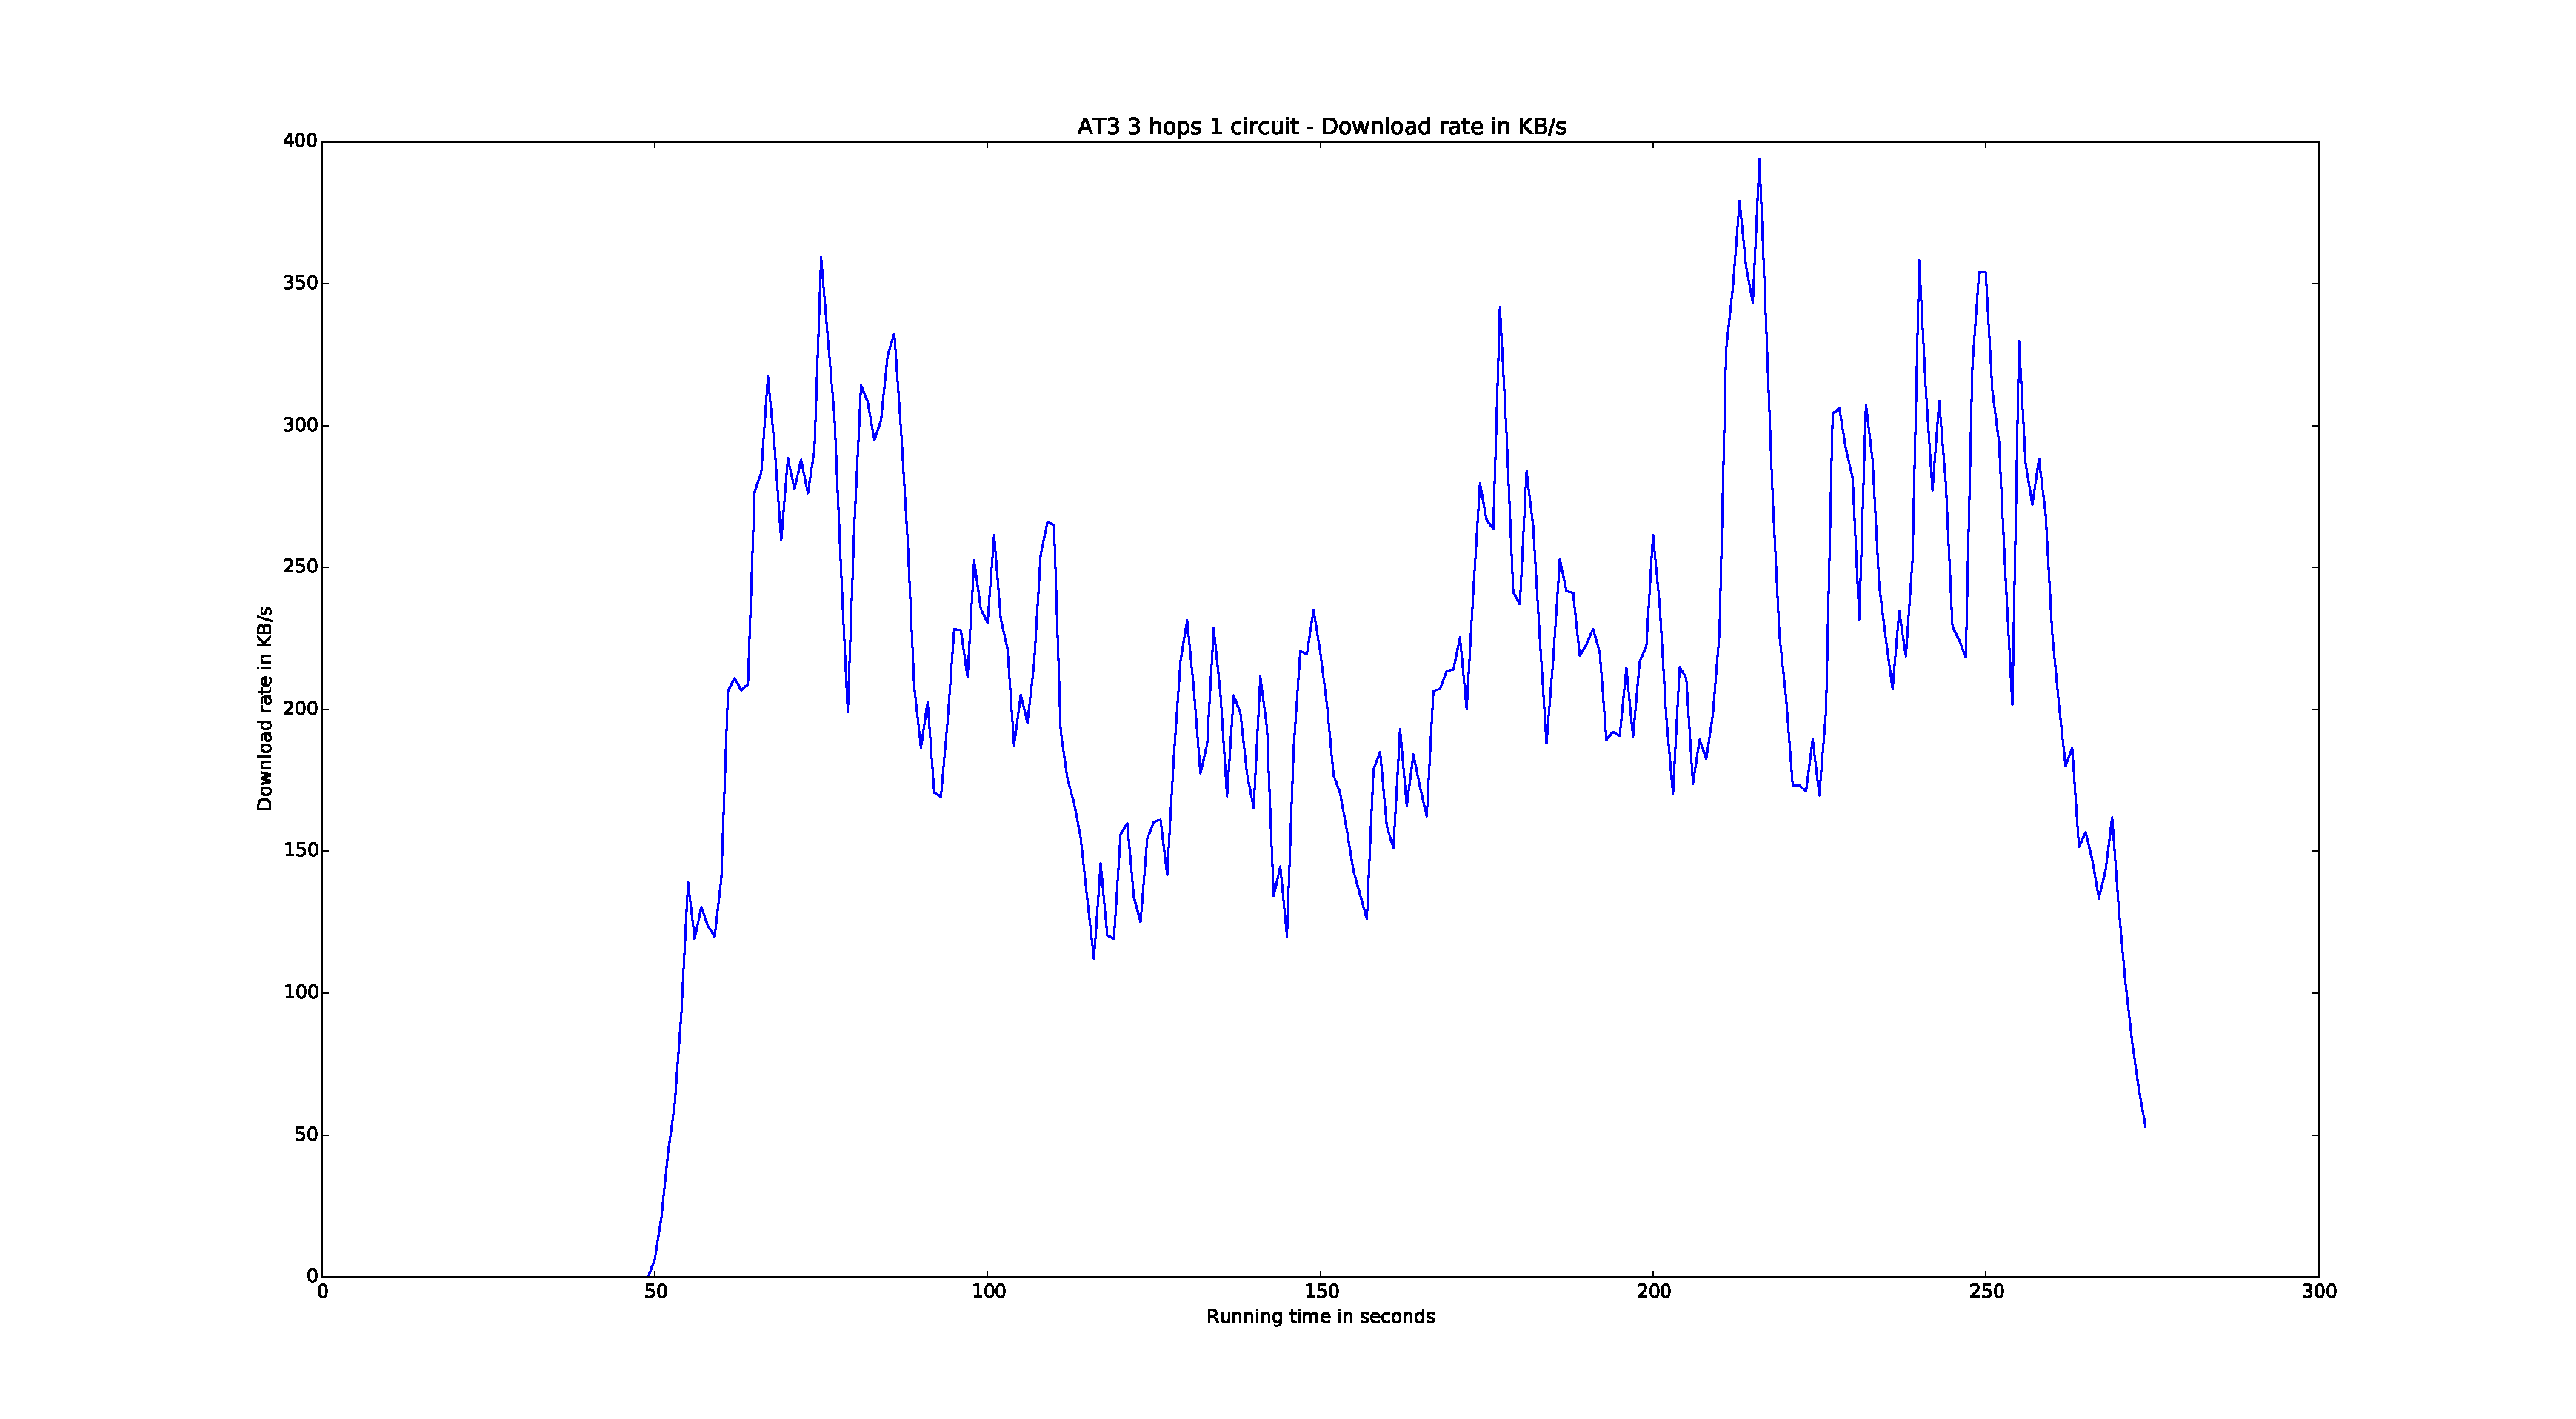
\includegraphics[width=\textwidth]{graphics/download_rate_3_hops_1_circuit.pdf}
 				\caption{The download rate of downloading a 50 MB over three hops with one circuits.}
 				\label{fig:download_rate_3_hops_1_circuit}
 			\end{figure*}
 			
 		\subsection{Download rate when downloading over 3 hops with 3 circuits}
 			To finish, we also measured the download rates when downloading with three hops and three circuits. Since encryption is also disabled here, we expect an increased download rate and thus a shorter download time. When we look at figure \ref{fig:download_rate_3_hops_3_circuits}, we see peaks reaching almost 500 KB/s and the download time being much shorter, confirming our expectations.
 			
 		\begin{figure*}[!htb]
			\centering
			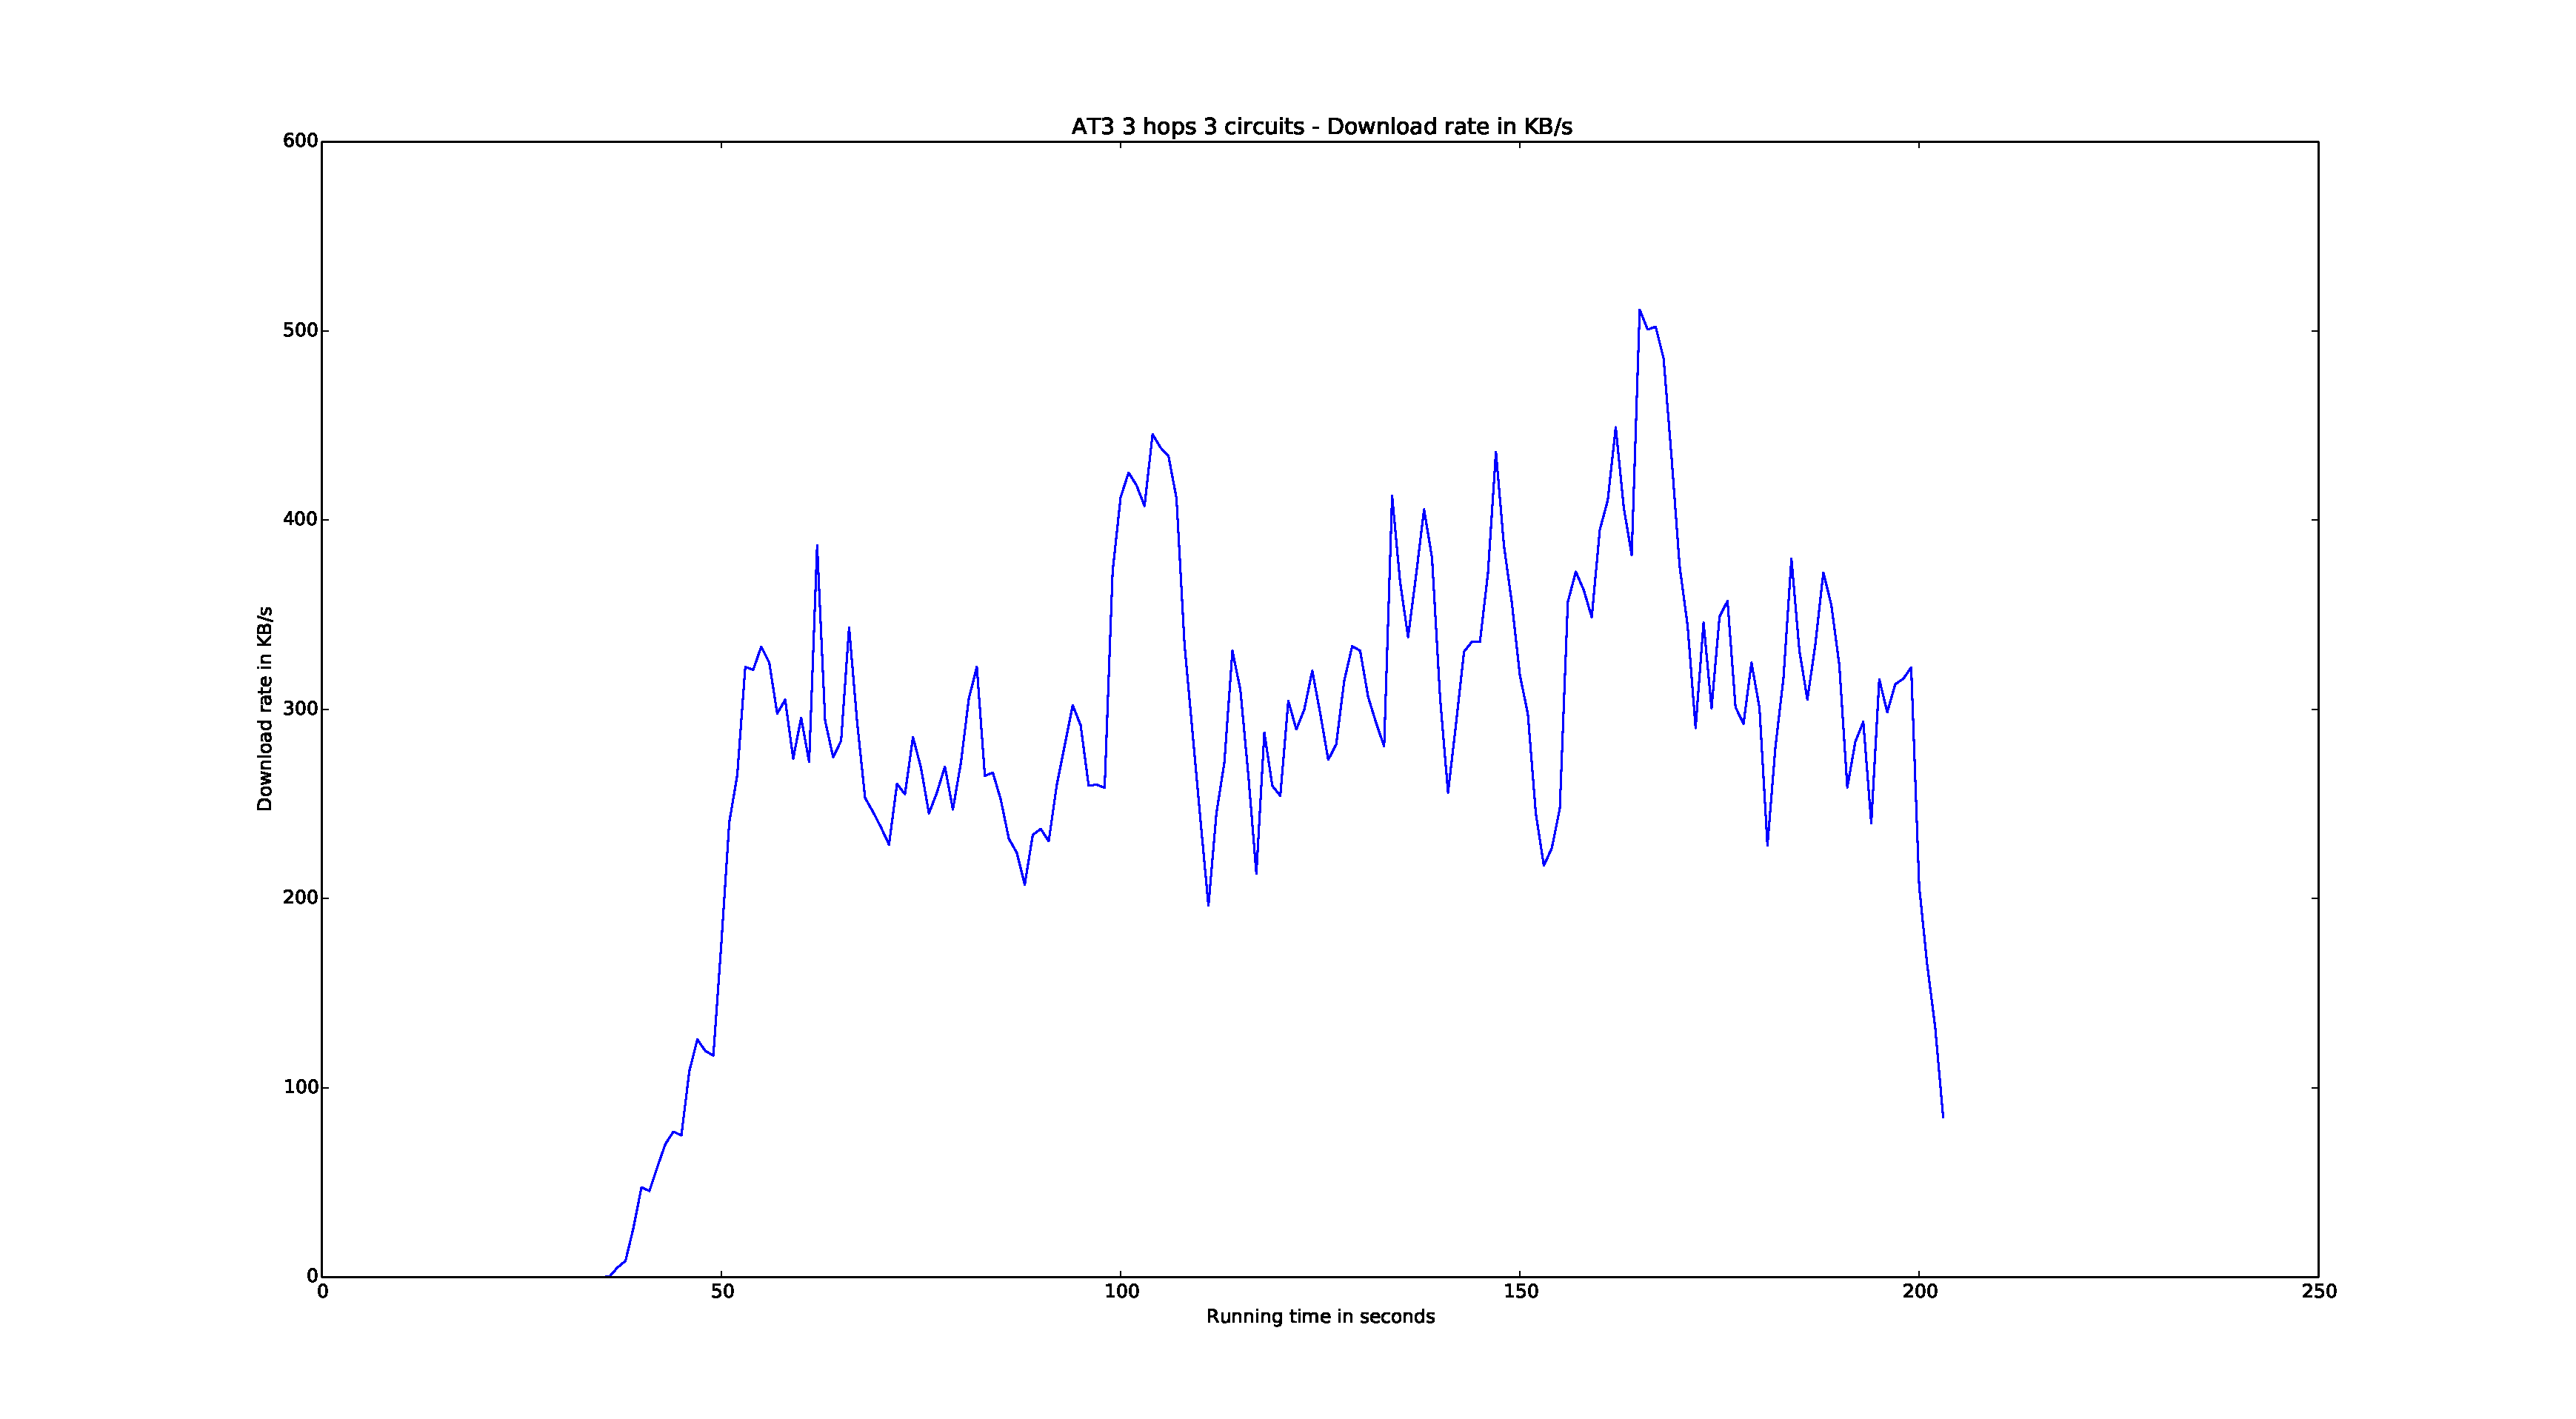
\includegraphics[width=\textwidth]{graphics/download_rate_3_hops_3_circuits.pdf}
			\caption{The download rate of downloading a 50 MB over three hops with one circuits.}
			\label{fig:download_rate_3_hops_3_circuits}
		\end{figure*}
		
\newpage